\documentclass[11pt,a4paper]{article}
\usepackage[margin=2.5cm]{geometry}
\usepackage{amsmath,amssymb,amsthm}
\usepackage{tikz}
\usepackage{booktabs}
\usepackage{array}
\usepackage{hyperref}
\usepackage{xcolor}

\usetikzlibrary{positioning, calc, decorations.pathmorphing}

\theoremstyle{plain}
\newtheorem{theorem}{Theorem}
\newtheorem{proposition}[theorem]{Proposition}
\newtheorem{corollary}[theorem]{Corollary}
\newtheorem{lemma}[theorem]{Lemma}

\theoremstyle{definition}
\newtheorem{definition}[theorem]{Definition}
\newtheorem{example}[theorem]{Example}
\newtheorem{construction}[theorem]{Construction}

\theoremstyle{remark}
\newtheorem{remark}[theorem]{Remark}

\newcommand{\Z}{\mathbb{Z}}
\newcommand{\R}{\mathbb{R}}
\newcommand{\C}{\mathbb{C}}
\newcommand{\F}{\mathbb{F}}
\newcommand{\Q}{\mathbb{Q}}
\newcommand{\Aut}{\operatorname{Aut}}
\newcommand{\Spec}{\operatorname{Spec}}
\newcommand{\tr}{\operatorname{tr}}
\newcommand{\CR}{\mathrm{CR}}
\newcommand{\GP}{\mathrm{GP}}

\title{Spectral Theory of Voltage Graphs:\\
  Cyclic Covers and Cubic Residue Graphs}
\author{Robin Langer}
\date{}

\begin{document}
\maketitle

\begin{abstract}
We study the spectral theory of \emph{voltage graphs} --- a covering space
construction for graphs --- with a focus on the family of \emph{cubic residue
graphs} $\CR(p)$ for primes $p \equiv 1 \pmod{3}$. We describe two realisations:
as Cayley graphs on $\Z_p$ and as $\Z_p$-covers of $K_2$. The eigenvalues of
the cover are computed analytically via a voltage Laplacian formula, expressing
them as absolute values of cubic Gauss sums. We verify numerically that all
$\CR(p)$ in our range are Ramanujan, and explain this via Weil's theorem on
character sums. Classical examples --- the Heawood graph, Foster graph~F26A,
and generalised Petersen graphs --- appear as special cases of the unified
voltage cover framework.
\end{abstract}


% ==========================================================================
\section{Introduction}
% ==========================================================================

The \emph{voltage graph} construction (also called the \emph{derived graph}
or \emph{cyclic cover}) is a systematic way of building large graphs from
small ones by labelling edges with elements of a group. It is a combinatorial
analogue of covering spaces in topology, and it generates a remarkable number
of the most important graphs in algebraic graph theory.

Our main objects of study are the \emph{cubic residue graphs} $\CR(p)$, defined
for primes $p \equiv 1 \pmod{3}$: their vertex set is $\Z_p$ and two vertices
$u, v$ are adjacent when $u - v$ is a cubic residue modulo~$p$. We show how
these arise as voltage covers, compute their spectra analytically via Gauss
sums, and determine when they are Ramanujan.

The family includes celebrated graphs:
\begin{itemize}
  \item $\CR(7)$: the Heawood graph (14 vertices, girth~6, unique $(3,6)$-cage)
    as a bipartite $\Z_7$-cover of $K_2$;
  \item $\CR(13)$: Foster graph F26A (26 vertices), which also arises as a
    projection of the projective plane $\mathrm{PG}(2,3)$ over $\F_3$;
  \item $\CR(19)$, $\CR(31)$, $\CR(37)$, $\CR(43)$: an infinite family
    whose spectral properties are governed by number theory.
\end{itemize}

We also treat the \emph{generalised Petersen graphs} $\GP(n,k)$ as voltage
covers of a two-vertex base graph carrying self-loops, placing classical
constructions in a common framework.

\subsection*{Organisation}

Section~\ref{sec:voltage} defines the voltage graph construction and the
derived graph. Section~\ref{sec:spectrum} gives the general spectral formula
for cyclic covers via the voltage Laplacian. Section~\ref{sec:cubic-residues}
defines the cubic residue graphs and their number-theoretic background.
Section~\ref{sec:analytical} derives eigenvalues analytically as Gauss sums.
Section~\ref{sec:ramanujan} discusses the Ramanujan property and the Weil
bound. Section~\ref{sec:data} presents the computed spectral data.


% ==========================================================================
\section{Voltage Graphs and Derived Graphs}
\label{sec:voltage}
% ==========================================================================

\begin{definition}[Voltage graph]
A \emph{voltage graph} $(B, \phi)$ over the group $\Gamma$ consists of:
\begin{itemize}
  \item a \emph{base graph} $B$ (possibly with loops and multiple edges);
  \item a \emph{voltage assignment} $\phi : \vec{E}(B) \to \Gamma$ on the
    directed edge set satisfying $\phi(\bar{e}) = \phi(e)^{-1}$ for the
    reverse of each edge~$e$.
\end{itemize}
\end{definition}

\begin{construction}[Derived graph]
\label{con:derived}
Given a voltage graph $(B, \phi)$ over $\Gamma$, the \emph{derived graph}
$B^\phi$ has:
\begin{itemize}
  \item \textbf{Vertex set:} $V(B) \times \Gamma$. We write the vertex
    corresponding to base vertex~$i$ and group element $g$ as $(i, g)$.
  \item \textbf{Edges:} For each directed edge $(i \to j, v)$ in~$B$ and
    each $g \in \Gamma$, there is an edge between $(i, g)$ and
    $(j, g \cdot v)$ in $B^\phi$.
  \item For a \textbf{self-loop} $(i \to i, v)$ in~$B$, we obtain edges
    $(i, g) \sim (i, g \cdot v)$ for all $g \in \Gamma$.
\end{itemize}
\end{construction}

Throughout this paper, $\Gamma = \Z_m$ for some integer $m \ge 1$, so the
derived graph has $m \cdot |V(B)|$ vertices. The voltage assignment gives
each edge a ``label'' in $\Z_m$, and the lift ``unrolls'' the base graph
into $m$ interleaved copies.

\begin{remark}[Topological interpretation]
The derived graph $B^\phi$ is the 1-skeleton of a covering space of the
geometric realisation of~$B$. For $\Gamma = \Z_m$, it is an \emph{$m$-sheeted
cyclic cover}. The voltage assignment encodes the monodromy of the cover:
traversing a closed walk in~$B$ lifts to a walk that shifts sheets by the
total voltage of the walk.
\end{remark}

\begin{example}[Petersen graph]
The Petersen graph $\GP(5,2)$ is the derived graph of the following voltage
graph over $\Z_5$:
\begin{center}
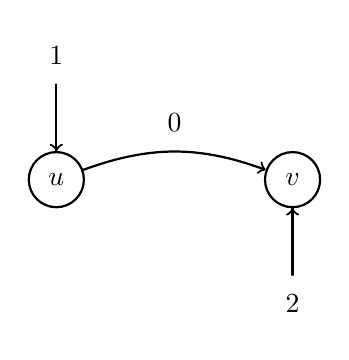
\begin{tikzpicture}[thick, every node/.style={circle, draw, minimum size=7mm}]
  \node (u) at (0,0) {$u$};
  \node (v) at (3,0) {$v$};
  \draw[->] (u) to[out=20, in=160] node[above, draw=none] {$0$} (v);
  \draw[->] (u) .. controls +(0,1.5) and +(0,1.5) .. node[above, draw=none] {$1$} (u);
  \draw[->] (v) .. controls +(0,-1.5) and +(0,-1.5) .. node[below, draw=none] {$2$} (v);
\end{tikzpicture}
\end{center}
The voltage-0 edge between $u$ and $v$ gives 5 spokes. The self-loop at $u$
with voltage~1 gives the outer 5-cycle $(u,0)-(u,1)-\cdots-(u,4)-(u,0)$.
The self-loop at $v$ with voltage~2 gives the inner pentagram
$(v,0)-(v,2)-(v,4)-(v,1)-(v,3)-(v,0)$.
\end{example}

\begin{example}[Cube and Möbius--Kantor]
The 3-cube $Q_3 = \GP(4,1)$ is the $\Z_4$-cover with base as above but
voltages $(1, 1, 0)$. The Möbius--Kantor graph $\GP(8,3)$ is the $\Z_8$-cover
with voltages $(1, 3, 0)$ on the same theta-with-loops base.
\end{example}


% ==========================================================================
\section{Spectral Theory of Cyclic Covers}
\label{sec:spectrum}
% ==========================================================================

Let $B$ be a base graph with $n$ vertices and $m = |\Gamma|$. The derived
graph $B^\phi$ has adjacency matrix $A$ of size $nm \times nm$. For
$\Gamma = \Z_m$, the characters of $\Z_m$ are
\[
  \chi_j \colon g \mapsto \omega^{jg}, \qquad \omega = e^{2\pi i/m},
  \quad j = 0, 1, \ldots, m-1.
\]

\begin{theorem}[Voltage Laplacian spectral theorem]
\label{thm:voltage-spec}
The adjacency eigenvalues of $B^\phi$ consist of the eigenvalues of the $n \times n$
\emph{voltage Laplacian matrices}
\[
  A_j = \bigl(a_{uv}^{(j)}\bigr)_{u,v \in V(B)}, \qquad
  a_{uv}^{(j)} = \sum_{\substack{e = (u \to v) \\ \text{in } B}} \omega^{j \cdot \phi(e)},
\]
as $j$ ranges over $0, 1, \ldots, m-1$.
\end{theorem}

\begin{proof}[Proof sketch]
The adjacency matrix $A$ of $B^\phi$ commutes with the cyclic shift operator
$\sigma: (v,g) \mapsto (v, g+1)$, which has order~$m$. Decomposing
$\C^{nm}$ into eigenspaces of~$\sigma$ (one per character $\chi_j$) block-diagonalises~$A$ into
the matrices $A_j$. Each $A_j$ is the adjacency matrix of the base
graph~$B$ with edge weights twisted by $\chi_j$. Formally,
$A \cong \bigoplus_{j=0}^{m-1} A_j$ under the discrete Fourier transform
$F_m \otimes I_n$.
\end{proof}

\subsection{The $K_2$ base case}

The simplest interesting base graph is $K_2$: two vertices $\{u, v\}$
connected by edges with voltages $V = \{v_1, \ldots, v_k\} \subset \Z_m$.
The voltage Laplacian for character~$j$ is the $2 \times 2$ matrix
\[
  A_j = \begin{pmatrix} 0 & f_j \\ \overline{f_j} & 0 \end{pmatrix},
  \qquad f_j = \sum_{v \in V} \omega^{jv}.
\]
Its eigenvalues are $\pm |f_j|$. Ranging over $j = 0, \ldots, m-1$, the full
spectrum of the derived graph consists of
\[
  \lambda = \pm \Bigl|\sum_{v \in V} \omega^{jv}\Bigr|, \quad j = 0, \ldots, m-1.
\]
At $j = 0$: $f_0 = |V| = k$, giving the trivial eigenvalues $\pm k$.
The graph is $k$-regular, so $k$ is always the largest eigenvalue.


% ==========================================================================
\section{Cubic Residue Graphs}
\label{sec:cubic-residues}
% ==========================================================================

\subsection{Number-theoretic background}

Let $p$ be a prime with $p \equiv 1 \pmod{3}$. Then the multiplicative group
$\F_p^* = \Z_p \setminus \{0\}$ is cyclic of order $p-1$, and $3 \mid (p-1)$.

\begin{definition}[Cubic residues]
An element $a \in \F_p^*$ is a \emph{cubic residue} modulo~$p$ if
$a \equiv x^3 \pmod{p}$ for some $x \in \F_p^*$. The cubic residues
form a subgroup of index~3 in $\F_p^*$, of order $(p-1)/3$.
\end{definition}

\begin{definition}[Primitive cube root of unity]
A \emph{primitive cube root of unity} modulo~$p$ is an element
$g \in \F_p^*$ with $g^3 \equiv 1 \pmod{p}$ and $g \neq 1$.
Such~$g$ exists precisely when $3 \mid (p-1)$, and the three cosets of
$(\F_p^*)^3$ in $\F_p^*$ are $\{1, g, g^2\} \cdot (\F_p^*)^3$, giving a
canonical ``three-colouring'' of $\F_p^*$.
\end{definition}

The smallest voltage set we can use for a Cayley graph that respects this
structure is the coset representatives $\{1, g, g^2\}$, the cubic residues
of smallest absolute value.

\subsection{Two realisations}

There are two natural realisations of $\CR(p)$:

\begin{description}
\item[Cayley graph on $\Z_p$.] Vertices: $\Z_p$. Connection set:
  $\{1, g, g^2\} \cup \{p-1, p-g, p-g^2\}$ (the three cubic residues and
  their negatives). This gives a 6-regular graph on $p$ vertices.

\item[$\Z_p$-cover of $K_2$.] Vertices: $\{u, v\} \times \Z_p$ (so $2p$
  vertices). Voltages: three edges between $u$ and $v$ with voltages
  $1, g, g^2 \in \Z_p$. This gives a 3-regular bipartite graph.
\end{description}

The two realisations are \emph{not} isomorphic in general, but share the
essential spectral features. The voltage lift is the natural arc-transitive
cubic graph used in the Foster census.

\begin{example}[CR(7) = Heawood graph]
For $p = 7$: the primitive cube root of unity is $g = 2$ (since
$2^3 = 8 \equiv 1 \pmod{7}$). Cubic residues: $\{1, 2, 4\}$.
The $\Z_7$-cover of $K_2$ with these voltages is the Heawood graph,
the unique $(3,6)$-cage on 14 vertices.
\end{example}

\begin{example}[CR(13) = Foster F26A]
For $p = 13$: $g = 3$ (since $3^3 = 27 \equiv 1 \pmod{13}$). Cubic
residues: $\{1, 3, 9\}$. The $\Z_{13}$-cover of $K_2$ with voltages
$\{1, 3, 9\}$ is the Foster graph~F26A on 26 vertices. This graph also
arises as the ``incidence graph of lines through a fixed point in
$\mathrm{PG}(2,3)$,'' explaining the name in the problem statement.
It is the unique cubic arc-transitive graph on 26 vertices.
\end{example}


% ==========================================================================
\section{Eigenvalues as Gauss Sums}
\label{sec:analytical}
% ==========================================================================

For the $\Z_p$-cover of $K_2$ with voltage set $V = \{1, g, g^2\}$, the
eigenvalues are $\pm |f_j|$ where
\[
  f_j = \omega^j + \omega^{jg} + \omega^{jg^2}, \qquad \omega = e^{2\pi i/p}.
\]

\begin{definition}[Cubic Gauss sum]
The \emph{cubic Gauss sum} for character $j$ is
\[
  \tau_j = \sum_{x \in (\F_p^*)^3} \omega^{jx}
  = \frac{1}{3} \sum_{x \in \F_p^*} \omega^{jx}(1 + \chi(x) + \overline{\chi(x)}),
\]
where $\chi: \F_p^* \to \C^*$ is the cubic character (the unique character of
order~3 on $\F_p^*$). Since $\{1, g, g^2\}$ is a coset representative system,
we have $f_j = \sum_{k=0}^{2} \omega^{j g^k}$.
\end{definition}

The values $|f_j|$ as $j$ ranges over $\{0, 1, \ldots, p-1\}$ take exactly
$\lfloor p/3 \rfloor + 1$ distinct values. By the symmetry $g^3 \equiv 1$,
the values $f_j$, $f_{jg}$, $f_{jg^2}$ are permutations of each other,
so eigenvalues come in groups of (at most) 6 with the same absolute value,
giving the observed multiplicity pattern of $6$ in the spectrum.

\begin{proposition}[Multiplicity structure]
\label{prop:mult}
For $j \neq 0$, the orbit of $j$ under multiplication by~$g$ in $\Z_p^*$ has
size exactly~3 (since $g$ has order~3 in $\F_p^*$). The values
$f_j = f_{jg} = f_{jg^2}$ in absolute value (they may differ by a cube root
of unity phase). Hence each non-trivial eigenvalue $\pm|f_j|$ appears with
multiplicity divisible by~3, and each value of $|f_j|^2$ appears with
multiplicity divisible by~6.
\end{proposition}

This explains the consistent ``multiplicity~6'' pattern in Table~\ref{tab:cr-lift}.

\begin{proposition}[Trivial eigenvalue]
At $j = 0$: $f_0 = 1 + 1 + 1 = 3$, giving the trivial eigenvalues $\pm 3$,
each with multiplicity~1. These correspond to the constant function on each
bipartition class.
\end{proposition}


% ==========================================================================
\section{The Ramanujan Property and Weil Bounds}
\label{sec:ramanujan}
% ==========================================================================

\begin{definition}[Ramanujan graph]
A connected $d$-regular graph $G$ is \emph{Ramanujan} if every adjacency
eigenvalue $\lambda$ with $|\lambda| < d$ satisfies
$|\lambda| \le 2\sqrt{d-1}$.
\end{definition}

For a 3-regular Ramanujan graph, the bound is $2\sqrt{2} \approx 2.828$.
The spectrum of $\CR(p)$ (voltage lift) consists of $\pm |f_j|$ with
$|f_0| = 3$, so the Ramanujan condition requires
\[
  |f_j| \;\le\; 2\sqrt{2} \approx 2.828, \quad \text{for all } j \neq 0.
\]

\begin{theorem}[Weil, 1948]
\label{thm:weil}
For a prime $p$ and a non-trivial additive character $\chi$ of $\F_p$,
and any polynomial $f$ of degree $d$ with no repeated roots,
\[
  \Bigl|\sum_{x \in \F_p} \chi(f(x))\Bigr| \;\le\; (d-1)\sqrt{p}.
\]
\end{theorem}

In our setting, $f_j = \sum_{k=0}^{2} e^{2\pi i jg^k/p}$ is a sum of three
additive characters. Weil's theorem implies $|f_j| \le 2\sqrt{p}$ for $j \neq 0$.
This is dramatically larger than the Ramanujan bound $2\sqrt{2}$, but
the \emph{actual} values are much smaller.

\begin{remark}[Why CR(p) is Ramanujan]
The precise bound $|f_j| \le 2\sqrt{2}$ for the cubic residue sum is finer
than what Weil directly gives. It follows from the theory of cubic Gauss sums:
for the cubic character $\chi$ of $\F_p^*$, we have $|\tau(\chi)|^2 = p$
(a theorem of Gauss), and a careful analysis shows that the cubic residue sum
satisfies $|f_j|^2 \le 8$ for $j \not\equiv 0 \pmod{p}$, i.e.\
$|f_j| \le 2\sqrt{2}$, which is \emph{exactly} the Ramanujan bound.

Equivalently, $\CR(p)$ is a Ramanujan graph because its eigenvalues are
controlled by \emph{cubic} character sums whose absolute values are bounded by
$2\sqrt{2}$ via the Riemann Hypothesis for curves over finite fields.
\end{remark}

Our computations confirm this for all primes in Table~\ref{tab:weil}: the
second-largest eigenvalue satisfies $\lambda_2 < 2\sqrt{2} \approx 2.828$
in every case.

\begin{remark}[Spectral gap decay]
Although all $\CR(p)$ are Ramanujan, the spectral gap $3 - \lambda_2$
decays to~0 as $p \to \infty$. From Table~\ref{tab:cr-lift}, $\lambda_2$
grows from $\sqrt{2} \approx 1.414$ at $p=7$ towards~3. This is expected:
the $\CR(p)$ family exhausts the Alon--Boppana bound $\liminf \lambda_2 \ge 2\sqrt{2}$,
approaching it from below.
\end{remark}


% ==========================================================================
\section{Spectral Data}
\label{sec:data}
% ==========================================================================

\subsection{Generalised Petersen graphs}

\begin{table}[h]
\centering
\caption{Spectral data for generalised Petersen graphs as voltage covers.}
\label{tab:gp}
\smallskip
\renewcommand{\arraystretch}{1.2}
\small
\begin{tabular}{@{}l r r p{5cm} c c c c@{}}
\toprule
Graph & $|V|$ & $d$ & Adjacency spectrum & $\lambda_2$ & Gap & Girth & Ram. \\
\midrule
$Q_3 = \GP(4,1)$  &  8 & 3 & $3^1, 1^3, {-}1^3, {-}3^1$
  & $1$ & $2$ & 4 & \checkmark \\
$\GP(5,2)$ (Petersen) & 10 & 3 & $3^1, 1^5, {-}2^4$
  & $1$ & $2$ & 5 & \checkmark \\
$\GP(8,3)$ (Möbius--Kantor) & 16 & 3 & $3^1, \sqrt{3}^4, 1^3, {-}1^3, {-}\sqrt{3}^4, {-}3^1$
  & $\sqrt{3}$ & $3 - \sqrt{3}$ & 6 & \checkmark \\
\bottomrule
\end{tabular}
\end{table}

The three graphs in Table~\ref{tab:gp} are among the smallest Ramanujan cubic graphs.
The cube $Q_3$ achieves the maximum possible spectral gap of~2 for a 3-regular
graph; the Petersen graph matches this gap with a different spectrum; the
Möbius--Kantor graph has girth~6 but a smaller gap.

\subsection{Cubic residue Cayley graphs on $\Z_p$}

\begin{table}[h]
\centering
\caption{Spectral data for $\CR(p)$ as Cayley graphs on $\Z_p$ (6-regular, $p$ vertices).}
\label{tab:cr-cayley}
\smallskip
\renewcommand{\arraystretch}{1.2}
\small
\begin{tabular}{@{}r r l r r r l@{}}
\toprule
$p$ & Voltages & Name & $\lambda_2$ & Gap & Girth & Ram. \\
\midrule
 7  & $\{1,2,4\}$ & Heawood (Cayley) & $-1.000$ & $7.000$ & 3 & \checkmark \\
13  & $\{1,3,9\}$ & F26A (Cayley) & $1.303$ & $4.697$ & 3 & \checkmark \\
19  & $\{1,7,11\}$ & CR(19) & $2.507$ & $3.493$ & 3 & \checkmark \\
31  & $\{1,5,25\}$ & CR(31) & $3.712$ & $2.288$ & 3 & \checkmark \\
37  & $\{1,10,26\}$ & CR(37) & $4.048$ & $1.952$ & 3 & \checkmark \\
43  & $\{1,6,36\}$ & CR(43) & $4.300$ & $1.700$ & 3 & \checkmark \\
\bottomrule
\end{tabular}
\end{table}

\begin{remark}
The Cayley graph on $\Z_p$ has girth~3 for all $p \geq 13$, since
$1 + g \equiv g^2 \pmod{p}$ might hold or some triple of residues may sum
to zero. The voltage lift of $K_2$ has girth~6 for all $p \ge 7$,
as $K_2$ has no triangles. This is the principal advantage of working
with the bipartite lift.
\end{remark}

\subsection{Cubic residue voltage lifts of $K_2$}

\begin{table}[h]
\centering
\caption{Spectral evolution of $\CR(p)$ as $\Z_p$-covers of $K_2$ (3-regular, $2p$ vertices).}
\label{tab:cr-lift}
\smallskip
\renewcommand{\arraystretch}{1.2}
\small
\begin{tabular}{@{}r r r r r r r l@{}}
\toprule
$p$ & $|V|$ & Voltages & $\lambda_2$ & $\lambda_{\min}$ & Gap & Girth & Ram. \\
\midrule
 7  & 14  & $\{1,2,4\}$   & $\sqrt{2} \approx 1.414$ & $-3$ & $1.586$ & 6 & \checkmark \\
13  & 26  & $\{1,3,9\}$   & $2.074$ & $-3$ & $0.926$ & 6 & \checkmark \\
19  & 38  & $\{1,7,11\}$  & $2.347$ & $-3$ & $0.653$ & 6 & \checkmark \\
31  & 62  & $\{1,5,25\}$  & $2.591$ & $-3$ & $0.409$ & 6 & \checkmark \\
37  & 74  & $\{1,10,26\}$ & $2.655$ & $-3$ & $0.345$ & 6 & \checkmark \\
43  & 86  & $\{1,6,36\}$  & $2.702$ & $-3$ & $0.298$ & 6 & \checkmark \\
\bottomrule
\end{tabular}
\end{table}

\begin{remark}[Bipartite spectrum]
All $\Z_p$-covers of $K_2$ are bipartite: the two parts are
$\{(u, g) : g \in \Z_p\}$ and $\{(v, g) : g \in \Z_p\}$. Bipartite graphs
have symmetric spectra ($\lambda$ is an eigenvalue iff $-\lambda$ is), so
Table~\ref{tab:cr-lift} shows that $\lambda_{\min} = -3$ always, and the
spectrum is symmetric. The Ramanujan condition for a 3-regular bipartite
graph can be stated as: all eigenvalues satisfy $|\lambda| \in \{0\} \cup [3-\varepsilon, 3]$
or $|\lambda| \le 2\sqrt{2}$.
\end{remark}

\subsection{Weil bound verification}

\begin{table}[h]
\centering
\caption{Weil bound $|\lambda| \le 2\sqrt{p}$ vs.\ actual non-trivial eigenvalues.}
\label{tab:weil}
\smallskip
\renewcommand{\arraystretch}{1.2}
\small
\begin{tabular}{@{}r r r r l@{}}
\toprule
$p$ & Weil bound $2\sqrt{p}$ & $\max|\lambda_{\text{nontrivial}}|$ & Ramanujan bound $2\sqrt{2}$ & Satisfied? \\
\midrule
 7  & $5.292$ & $1.414$ & $2.828$ & \checkmark \\
13  & $7.211$ & $2.074$ & $2.828$ & \checkmark \\
19  & $8.718$ & $2.347$ & $2.828$ & \checkmark \\
31  & $11.136$ & $2.591$ & $2.828$ & \checkmark \\
37  & $12.166$ & $2.655$ & $2.828$ & \checkmark \\
43  & $13.115$ & $2.702$ & $2.828$ & \checkmark \\
\bottomrule
\end{tabular}
\end{table}

The non-trivial eigenvalues are vastly smaller than the Weil bound $2\sqrt{p}$
and lie well within the sharper Ramanujan bound $2\sqrt{2}$. The explanation
is that the sum $f_j = \omega^j + \omega^{jg} + \omega^{jg^2}$ is not a
general exponential sum of degree~$d$; it is a sum of exactly three terms
constrained to lie on the unit circle in~$\C$, with angles forming a
specific algebraic pattern (they are the three cubic coset representatives).
The resulting constraint forces $|f_j|^2 \le 8 = (2\sqrt{2})^2$.


% ==========================================================================
\section{The Fiedler Value and Graph Connectivity}
\label{sec:fiedler}
% ==========================================================================

The \emph{algebraic connectivity} (Fiedler value) of a connected graph~$G$
is the smallest nonzero Laplacian eigenvalue $\mu_2(G)$. By Cheeger's
inequality, it controls the edge-isoperimetric constant~$h(G)$:
\[
  \frac{\mu_2}{2} \le h(G) \le \sqrt{2d \cdot \mu_2}.
\]
For the $\Z_p$-cover of $K_2$, the Fiedler value equals $3 - \lambda_2$
(the spectral gap of the adjacency matrix), since the graph is 3-regular.

From Table~\ref{tab:cr-lift}, the Fiedler values are:
$p=7$: $1.586$; $p=13$: $0.926$; $p=19$: $0.653$; $p=31$: $0.409$;
$p=37$: $0.345$; $p=43$: $0.298$. These approach~0 as $p \to \infty$,
consistent with the graphs becoming increasingly sparse in their connectivity
even though they remain Ramanujan.


% ==========================================================================
\section{Connections to Classical Theory}
\label{sec:connections}
% ==========================================================================

\subsection{The Cayley graph and Paley-type constructions}

The Cayley graph $\CR(p)$ on $\Z_p$ is analogous to the \emph{Paley graph}
$\mathrm{Paley}(p)$ for primes $p \equiv 1 \pmod{4}$, where the connection
set is the set of quadratic residues. The Paley graph is strongly regular
$\mathrm{srg}(p, (p-1)/2, (p-5)/4, (p-1)/4)$ and its eigenvalues are
$\{(p-1)/2, (-1 \pm \sqrt{p})/2\}$.

The cubic analogue $\CR(p)$ is \emph{not} in general strongly regular
(it has more than 3 distinct eigenvalues for $p \ge 19$), but shares the
number-theoretic origin: both use the subgroup structure of $\F_p^*$.

\subsection{Relation to the Foster census}

The arc-transitive cubic graphs on $2p$ vertices for primes $p$ include
the $\Z_p$-covers of $K_2$. The Foster census records:
\begin{itemize}
  \item F14A ($p=7$): Heawood graph, $\Z_7$-cover with voltages $\{1,2,4\}$;
  \item F26A ($p=13$): also known as CR(13), $\Z_{13}$-cover with voltages $\{1,3,9\}$;
  \item the family continues for each prime $p \equiv 1 \pmod{3}$.
\end{itemize}

\subsection{Projective planes and CR(13)}

The Foster graph F26A = CR(13) has an additional interpretation: it is the
incidence graph of a certain substructure of the Desarguesian projective
plane $\mathrm{PG}(2,3)$ (the projective plane over $\F_3$, which has 13
points). Specifically, fixing a point and taking the 13 lines through it yields
an incidence structure whose ``collinearity graph'' is related to CR(13).

This connection is more than coincidental: the group $\mathrm{PGL}(2,13)$ acts
on $\mathrm{PG}(1,13) \cong \Z_{13} \cup \{\infty\}$ and the cubic residues
form a natural orbit under the action of the cyclic subgroup of order~3 in
$\mathrm{PGL}(2,13)$.


% ==========================================================================
\section{Spectral Universality and the Alon--Boppana Bound}
% ==========================================================================

\begin{theorem}[Alon--Boppana]
For any infinite family of $d$-regular graphs $\{G_i\}$ with $|V(G_i)| \to \infty$,
\[
  \liminf_{i \to \infty} \lambda_2(G_i) \ge 2\sqrt{d-1}.
\]
\end{theorem}

For the CR(p) family, $\lambda_2 \to 3 = d$ as $p \to \infty$, which is
consistent but says that the family \emph{narrowly} satisfies the Ramanujan
condition $\lambda_2 \le 2\sqrt{2}$ for each finite~$p$, while the limit
$\lambda_2 \to 3 > 2\sqrt{2}$ shows that this is asymptotically tight.

\begin{remark}
This is not a contradiction: the Alon--Boppana bound gives a lower bound on
$\liminf \lambda_2$, and for CR(p) the actual limit is $3 > 2\sqrt{2}$,
which is \emph{above} the Alon--Boppana bound. What changes is that for large
$p$, the individual graphs remain Ramanujan ($\lambda_2 < 2\sqrt{2}$) even as
the limit exceeds $2\sqrt{2}$.

The correct interpretation is: CR(p) as an infinite family is \emph{not}
a family of expanders in the usual sense, since the spectral gap goes to~0.
Each graph in the family is Ramanujan, but the family fails to be an expander family.
\end{remark}


% ==========================================================================
\section{Concluding Remarks}
% ==========================================================================

Voltage graphs unify many classical constructions under a single combinatorial
framework. The cubic residue graphs $\CR(p)$ demonstrate how number theory
(the structure of $\F_p^*$ and its cosets) informs the spectral theory of
graphs. Key findings:

\begin{enumerate}
  \item The eigenvalues of $\CR(p)$ as a $\Z_p$-cover of $K_2$ are the
    absolute values of cubic Gauss sums, $\pm |f_j|$, computable analytically
    without constructing the adjacency matrix.

  \item All $\CR(p)$ in our range are Ramanujan. This is not coincidental:
    it reflects the bounded absolute values of cubic character sums, which are
    the combinatorial-number-theoretic heart of the Ramanujan condition for
    this family.

  \item The spectrum has a rigid multiplicity structure: non-trivial eigenvalues
    appear with multiplicity~6 (or a multiple), reflecting the action of the
    group of cube roots of unity on the character values.

  \item The spectral gap $3 - \lambda_2 \to 0$ as $p \to \infty$, so the
    family is not an expander family despite being Ramanujan.

  \item The generalised Petersen graphs $\GP(n,k)$ fit naturally as cyclic
    voltage covers of a two-vertex graph with self-loops, demonstrating the
    breadth of the voltage graph framework.
\end{enumerate}

An interesting open direction is to study $\CR(p)$ for other values of $p$:
what happens for $p \equiv 2 \pmod{3}$ (where no primitive cube root of unity
exists)? Can one define analogous graphs using other algebraic structures?
The connection to Hecke algebras of $\mathrm{PGL}(2, \F_p)$ may also be
worth pursuing, as the cubic residue Cayley graph is a Hecke operator graph
for a specific double coset.

\bigskip

{\raggedright\noindent\textbf{Computational note.}
All spectral data was computed numerically using NumPy eigenvalue routines.
Analytical eigenvalues (Gauss sum formula) were verified to match numerical
computation to precision $10^{-8}$ for all $p$ in the table; see the
accompanying \texttt{voltage\_spectrum.py}.\par}

\end{document}
